\documentclass[12pt]{article}


\usepackage[a4paper, margin=2.5cm]{geometry}


\usepackage{graphicx}
\usepackage{float}
\usepackage{hyperref}



\begin{document}


\begin{abstract}
1.5/10, too much waffle.
\end{abstract}

\section*{Introduction}
In 2012, the ATLAS \cite{atlasann} and CMS \cite{cmsannouncement} collaborations at the Large Hadron Collider (LHC) announced the discovery of a new particle believed to be the Higgs boson. This was the culmination of over 50 years of theoretical and experimental work to complete the Standard Model of Particle Physics (SM), the mathematical theory which successfully predicted the existence and properties of two new quarks, the tau lepton, gluon and W and Z bosons as well as the Higgs \cite{smpredictions}. However, the question of whether this particle discovered is the Higgs predicted in the Standard Model remains, which has led to an ongoing study of its properties and couplings to other particles. These studies, should any discrepancy be found, would give evidence for new physics beyond the Standard Model, and possibly help to explain some of the holes in the current theories such as the existence of dark matter and neutrino oscillations.

The Higgs boson is a scalar (spin 0) boson with a variety of production and decay modes from SM particles. At the LHC, the primary production mode is gluon fusion, followed by vector boson fusion (VBF) \cite{higgsproduction}. 

\begin{figure}[H]
\centering
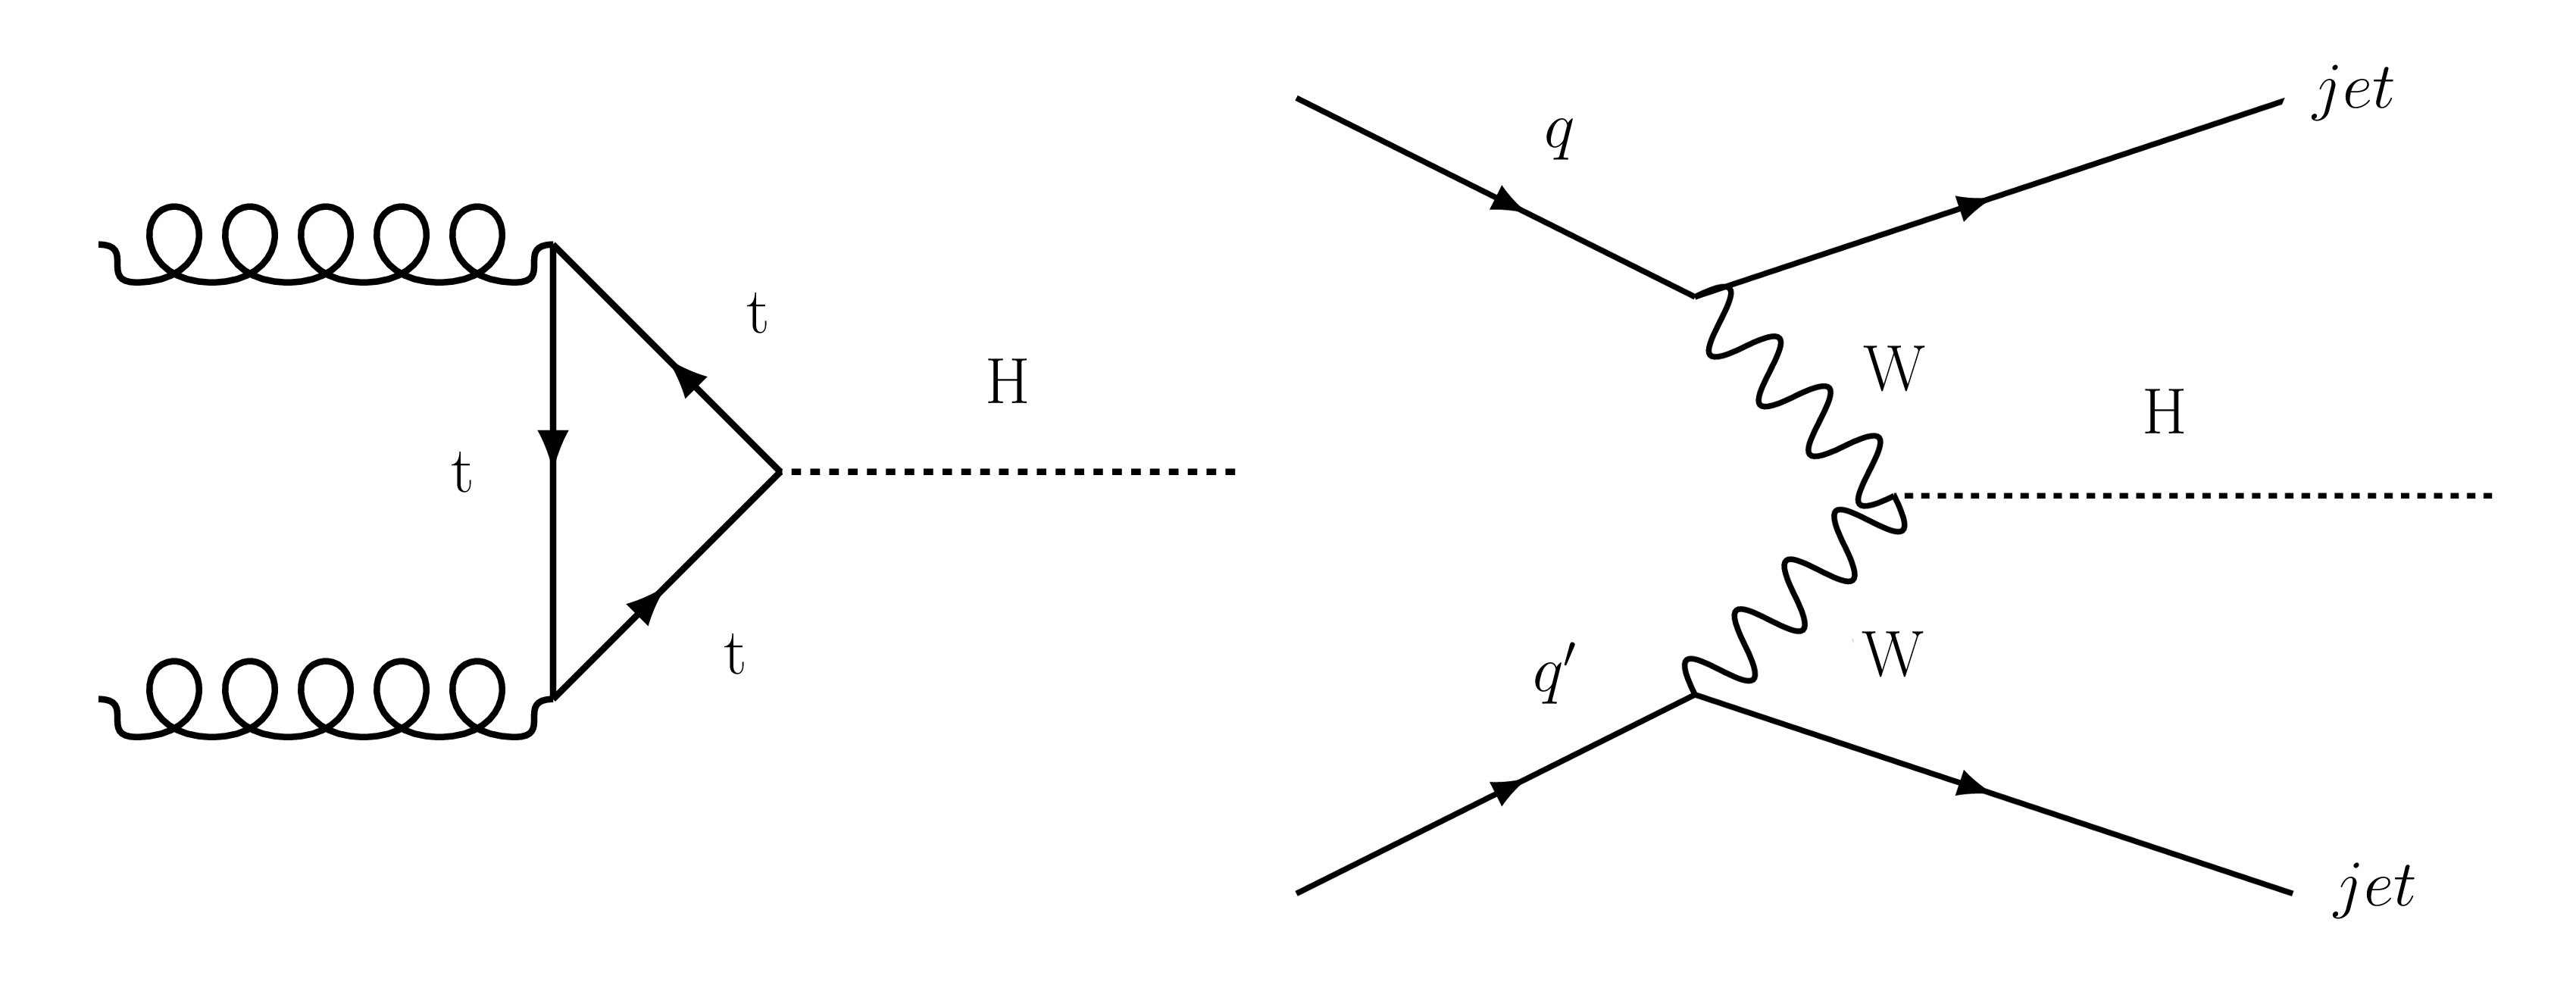
\includegraphics[width=12cm]{form.png}
\caption{Feynman diagrams for gluon fusion (left) and vector boson fusion (right). The forward jets from VBF can be used to identify it as the production mode compared to other modes. (Created using \cite{feynmanmaker}).}
	\label{form}
\end{figure}

Alternative production modes include associated production with a W boson and the recently observed associated production with top quarks \cite{tth}. These modes are all individually useful as they have distinct signatures and can be used to probe the couplings of the Higgs with the different particles involved. 

The decay modes of the SM Higgs include decays into vector bosons, two tau leptons, two b quarks and two photons \cite{gluinotheory1}, which is the decay mode which will be considered in this project. Despite having a relatively small cross-section \cite{cmsannouncement}, the diphoton mode has the advantage of being a very clean mode, since the photons do not produce jets. It also has very good mass resolution, since all the decay products are visible, so the invariant mass of the photons gives a sharp peak \cite{seezdiphoton}. These positives led to the mode being identified as one of the most promising for discovering the Higgs. Additionally, the diphoton decay is interesting since it proceeds via a loop process, due to the photon being massless and therefore having no direct coupling to the Higgs. This makes this decay mode more sensitive to interference effects and therefore the fermion coupling strengths \cite{cmsanalysis1}.  The existence of this mode is also significant since it excludes spin 1 models for the Higgs by conservation of spin angular momentum. 

\begin{figure}[H]
\centering
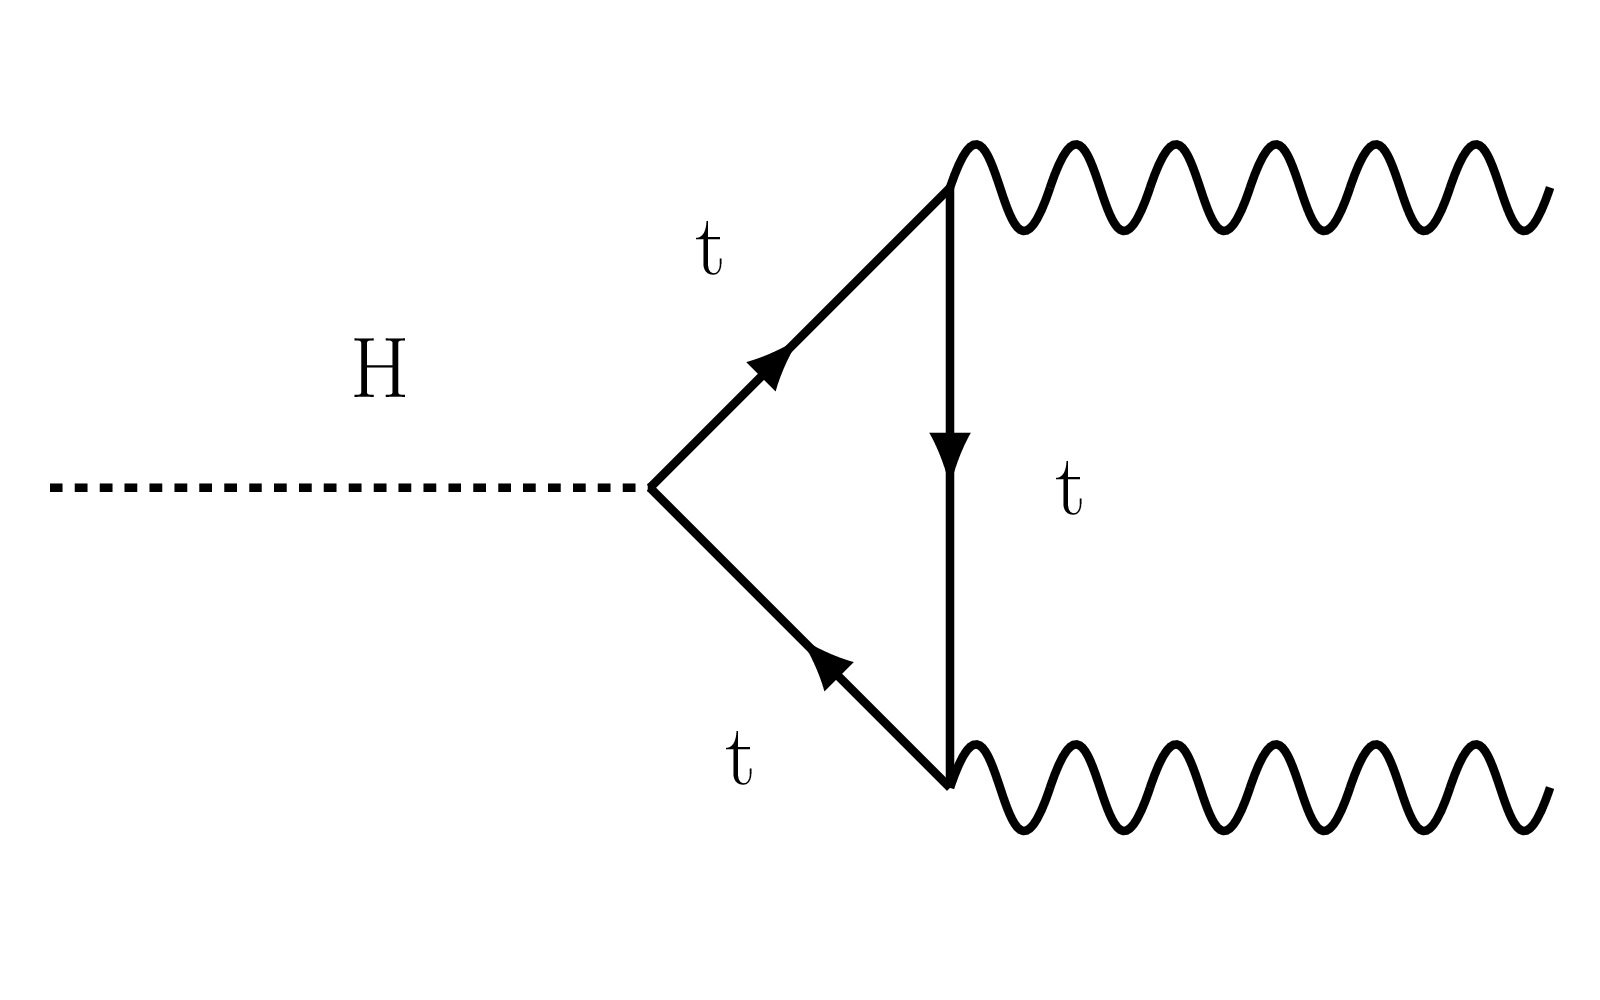
\includegraphics[width=6cm]{decay.png}
\caption{One of the possible feynman diagrams for the diphoton decay via a top quark loop. Another possibiliy is a W boson loop, so these two modes will interfere. (Created using \cite{feynmanmaker}).}
	\label{decay}
\end{figure}




Simplified template cross sections are a method for interpreting data first used LHC run 1, where the cross sections of each production mode are split into multiple 'bins', mutually exclusive areas of phase space, in order to systematically reduce the theory dependence of results. This can help reduce the theoretical uncertainties associated with measured values, as well as removing the dependencies on the underlying physics model being used, something that is particularly helpful when looking for beyond-the-standard-model (BSM) physics. 

With the large volumes of data the LHC produces and will continue to produce, finding a way to make this data more manageable is important. In recent years, machine learning has increased in popularity as a tool to do this. These algorithms can be trained to identify event signatures based on a set of criteria against the expected backgrounds for a signal, allowing them to distinguish between an interesting event and an uninteresting event and thus decreasing the number of events stored for further analysis. With the integrated luminosity of the LHC increasing with each upgrade, machine learning techniques become even more important, with increased pileup (more interactions occurring in the detector at once) making it harder to separate out individual events. 

The aim of this project is to analyse and improve the current machine learning techniques being used at CMS in H$\rightarrow \gamma\gamma$, in order to increase its usage for event selection and categorisation into the `bins' defined by the simplified template cross section method, as well as potentially looking at how the current binning choices and setup could be improved for future data analyses. This will allow better measurement of the Higgs boson's properties, allowing for more detailed tests of the SM-like Higgs discovered and further probing for BSM physics in the diphoton decay. 

\section*{Background material}

\subsection*{Theory}

In the 1960s, particle physics theory was attempting to describe the weak force using gauge theories, where the Lagrangian of a system is invariant under certain transformations. Spontaneous symmetry breaking is where a system in the ground state does not have the same symmetry as the Lagrangian that describes it. This is observed in nature, so theories needed to include it, but the physical origin of the breaking remains a mystery. Including this broken symmetry in gauge theories and quantising the fields predicted the existence of `gauge' bosons such as the W and Z. 

However, breaking the symmetry in this way requires all bosons to be massless due to Goldstone's theorem \cite{higgstheory}, giving rise to so-called `Goldstone' bosons. This presents a problem as the weak force is known to have a very short range, so any mediator particles are required to be massive.

The first step towards a solution was provided by Schwinger in 1964 \cite{theory1}, who only considered the non-relativistic case. This was followed by Englert and Brout \cite{theory2}, Higgs \cite{higgstheory} and Guralnik, Hagen and Kibble \cite{theory3}. Their insights were that introducing a new scalar field to break the symmetry, rather than requiring the existing fields to have broken symmetry, allowed the W and Z bosons to acquire mass by `absorbing' three of the four degrees of freedom corresponding to bosons \cite{theory4}. The Higgs boson is the fourth degree of freedom, and is the excitation of this new scalar field. The photon remains massless as it corresponds to the unbroken part of the electroweak symmetry and is thus not a Goldstone boson \cite{theory5}. This theory does not predict the mass of the Higgs boson, rather it is a parameter that if known allows all the expected coupling strengths to be predicted. 

It was later observed by Weinburg that via a Yukawa interaction (an interaction between a scalar field like the Higgs field and a Dirac field, which describes the behaviour of fermions) this would also give mass to fermions \cite{lepmass}. Combining the unified electroweak model with this new information produces what is now referred to as the Standard Model of Particle Physics. 

\subsection*{The discovery and beyond}
The first focussed search for the Higgs boson began in the 1990s. The Large Electron Positron Collider (LEP) at CERN and the Tevatron at Fermilab were able to set limits on the Higgs mass and couplings to SM particles \cite{limit1} \cite{limit3p5} \cite{limit3}. Then in early 2012, the CMS and ATLAS collaborations analysed the first data run of the LHC and saw an excess of events in the diphoton channel, ATLAS at 2.8 standard deviations \cite{limit6} and CMS at 3.1 $\sigma$ \cite{limit7}. Both collaborations improved their analyses by combining more decay channels, ATLAS finally reporting an excess at 126.0$\pm$0.6 GeV with significance of 5.9 sigma \cite{atlasann} and CMS saw an excess at 125.3$\pm$0.6 GeV at 5.0 sigma \cite{cmsannouncement}. 


Both of these analyses confirmed the existence of a new particle, which now needed further scrutiny to determine if it was the SM Higgs, including verifying the new boson's decay and production modes and checking for properties such as spin-0 or even parity. The observation of the diphoton decay mode excluded spin-1 hypotheses, and a later hypothesis test between spin-0 and spin-2 disfavoured the spin-2 hypothesis at the 95$\%$ confidence level \cite{cmsupdate2}. Even parity was confirmed tentatively at first \cite{parity1}, but combined with the spin-0 results negative parity was disfavoured at 99$\%$ CL \cite{parity2}. 

For each of the production and decay modes, a variable $\sigma$/$\sigma_{SM}$ is defined to test compatibility with the SM, referred to as $\mu$. This is expected to be close to 1, and indeed all measurements of it so far have been consistent with the SM Higgs \cite{atlasann}\cite{cmsupdate2}. The diphoton, four lepton and vector boson modes had already been observed, but in 2014 the decay to two tau leptons was observed \cite{taudecayproof} and most recently the decay to two b quarks has been confirmed \cite{bbdecayproof}. Some expected decays, such as the decay to gluons \cite{gluinotheory2} have not yet been observed, while the absence of others such as the H $\rightarrow$ Z$\gamma$ decay have disfavoured hypotheses such as the composite Higgs \cite{comp} and a different particle masquerading as the Higgs \cite{impostor}.

\subsection*{Methodology of the diphoton channel}
The expected signature of a H $\rightarrow \gamma\gamma$ decay is a narrow peak above the background found in the mass spectrum of the two photon system \cite{sethpresentation}. The observation of this has two main stages - the identification of the photons, and the measurement of their properties in order to reconstruct the decay. In the first stage, energy deposits in the electromagnetic calorimeter (ECAL) consistent with a photon are looked for. If an event has two of these, they then need to be analysed further to make sure that the particles are photons, since electrons and fragments from hadron jets such as $\pi^{0}$ will leave similar deposits \cite{recon}. To do this, a set of criteria called `Photon identification' are developed. To find the invariant mass of the photon pair, the angles of the decay are needed, so the point of decay needs to be reconstructed (as the photons don't leave any deposits in the inner part of the detector). This is difficult, since it can only be done statistically, and any errors in the vertex position will increase the width of the mass peak \cite{review1}. Another uncertainty which could increase the width are imperfect energy measurements in the ECAL, but these can be corrected for \cite{cmslimits}. Finally, additional criteria designed to differentiate between a Higgs decay and a background decay are applied to the data. The main background in this decay channel is QCD production of two photons, and is irreducible \cite{atlaslimits}. 

Thus, as well as working on upgrading the LHC and the detectors themselves, the methods of photon identification, reconstruction and signal/background identification have needed improvements with each data run and are still being improved currently \cite{cms13tev1}. With improvements to the LHC itself, an additional challenge is presented by the increase in integrated luminosity and thus increased pileup, which has led to greater need for better data processing methods such as machine learning.


\subsection*{Machine learning methods}

Generally, the aim for any machine learning algorithm being used on LHC data is to cut away as much uninteresting data as possible. This could be right after data collection, with bad quality events being discarded, or the identification of particles based on the tracks left in the detector and separation from any expected backgrounds. The pattern recognition abilities of machine learning algorithms appear to be an efficient way to do this. 

Initially, the most commonly used algorithm used for this was boosted decision trees (BDTs) \cite{ml7}. Here, each input variable is a `node', and the algorithm makes multiple cuts on these until some predefined end point is reached. The cuts are across multiple variables at once, and are chosen to maximise the change in some classifying variable, for example the signal-to-background ratio of a sample. Once this is completed, each point in the sample space is classified as either `signal' or 'background' and the background data can be discarded if needed. One problem with this method is that it is very sensitive to the initial setup, as small statistical fluctuations in the training data can have a large impact. The solution to this is to use `boosting', where multiple decision trees are combined to reduce the errors and increase the overall stability \cite{ml8}. BDTs have been used successfully in experiments such as MiniBooNE \cite{ml2}, and are good at handling large data inputs, but even with the boosting are still not massively robust and can have issues with overfitting, where the tree created is specialised to the training data and doesn't work with real data as well \cite{ml1}. 

Both CMS and ATLAS have used BDTs in their analyses in a variety of different ways. For example, using a BDT to identify tau leptons in decays compared to electrons and jets has been implemented in ATLAS, with tests confirming the expected score distributions when run on different sets of simulated data \cite{ml4}. Similarly, ATLAS has also tested b quark tagging using BDTs, and in Run 2 has been using the algorithms to distringush between b jets and c jets \cite{ml5}. CMS made extensive use of BDTs during Run 1, using them for photon identification, uncertainty estimation and photon energy correction. This final tree was trained on simulated data with a known true energy and a `measured' raw energy, with the BDT aiming to get the corrected value as close to the true value as possible without using the information itself \cite{ml6}. Using a BDT allowed the photons to be classified by signal purity, allowing an additional analysis to be done on a smaller sample of data. The impact of this was estimated to be equal to collecting 50$\%$ more data \cite{mlreview}.


These successes show machine learning in general is a useful tool in high energy physics, and has led to the BDTs being continuously optimised and improved during both runs of the LHC so far. 

However, in recent years, the improvements in BDTs for LHC data have started to slow down, leading to more research into different types of machine learning which may be more effective. One class of algorithms that has received much interest recently is Deep Learning. This differs from `shallow' methods in that it teaches itself how to spot the features in the data from the raw data rather than being told how to spot them. This makes them much more versatile than shallow methods and can lead to the algorithm itself finding better distinguishing features between, say, a signal and a background event, than the current set being used. It can also create a set of criteria with a greater number of inputs more easily than current methods, which only use a few variables chosen based on human knowledge and discard the rest. The discarded data could contain extra information for the algorithm, so including more variables could make the identification better. These algorithms can be trained in two different ways; aided, where the training data is labelled to show what the features mean, and unaided, where the training data is unlabelled and the algorithm is left to make its own decisions about the significances of things. 

(previous sucesses and searches)

 


\subsection*{Developments of simplified template cross sections}
atlas are ahead of us, booooooooo. 

\section*{Conclusion}



\bibliography{bv1}{}
\bibliographystyle{unsrt}
\end{document}

%After having read a review of the literature, a reader should have a rough idea of:
%the major achievements in the reviewed field,
%the main areas of debate, and
%the outstanding research questions.








